
%% bare_conf.tex
%% V1.3
%% 2007/01/11
%% by Michael Shell
%% See:
%% http://www.michaelshell.org/
%% for current contact information.
%%
%% This is a skeleton file demonstrating the use of IEEEtran.cls
%% (requires IEEEtran.cls version 1.7 or later) with an IEEE conference paper.
%% Support sites:
%% http://www.michaelshell.org/tex/ieeetran/
%% http://www.ctan.org/tex-archive/macros/latex/contrib/IEEEtran/
%% and
%% http://www.ieee.org/

%%*************************************************************************
%% Legal Notice:
%% This code is offered as-is without any warranty either expressed or
%% implied; without even the implied warranty of MERCHANTABILITY or
%% FITNESS FOR A PARTICULAR PURPOSE! 
%% User assumes all risk.
%% In no event shall IEEE or any contributor to this code be liable for
%% any damages or losses, including, but not limited to, incidental,
%% consequential, or any other damages, resulting from the use or misuse
%% of any information contained here.
%%
%% All comments are the opinions of their respective authors and are not
%% necessarily endorsed by the IEEE.
%%
%% This work is distributed under the LaTeX Project Public License (LPPL)
%% ( http://www.latex-project.org/ ) version 1.3, and may be freely used,
%% distributed and modified. A copy of the LPPL, version 1.3, is included
%% in the base LaTeX documentation of all distributions of LaTeX released
%% 2003/12/01 or later.
%% Retain all contribution notices and credits.
%% ** Modified files should be clearly indicated as such, including  **
%% ** renaming them and changing author support contact information. **
%%
%% File list of work: IEEEtran.cls, IEEEtran_HOWTO.pdf, bare_adv.tex,
%%                    bare_conf.tex, bare_jrnl.tex, bare_jrnl_compsoc.tex
%%*************************************************************************

% *** Authors should verify (and, if needed, correct) their LaTeX system  ***
% *** with the testflow diagnostic prior to trusting their LaTeX platform ***
% *** with production work. IEEE's font choices can trigger bugs that do  ***
% *** not appear when using other class files.                            ***
% The testflow support page is at:
% http://www.michaelshell.org/tex/testflow/

% Also note that the "draftcls" or "draftclsnofoot", not "draft", option
% should be used if it is desired that the figures are to be displayed in
% draft mode.
%
\documentclass[conference]{IEEEtran}


% Some very useful LaTeX packages include:
% (uncomment the ones you want to load)


% *** MISC UTILITY PACKAGES ***
%
%\usepackage{ifpdf}
% Heiko Oberdiek's ifpdf.sty is very useful if you need conditional
% compilation based on whether the output is pdf or dvi.
% usage:
% \ifpdf
%   % pdf code
% \else
%   % dvi code
% \fi
% The latest version of ifpdf.sty can be obtained from:
% http://www.ctan.org/tex-archive/macros/latex/contrib/oberdiek/
% Also, note that IEEEtran.cls V1.7 and later provides a builtin
% \ifCLASSINFOpdf conditional that works the same way.
% When switching from latex to pdflatex and vice-versa, the compiler may
% have to be run twice to clear warning/error messages.



% *** CITATION PACKAGES ***
\usepackage{cite}
% cite.sty was written by Donald Arseneau
% V1.6 and later of IEEEtran pre-defines the format of the cite.sty package
% \cite{} output to follow that of IEEE. Loading the cite package will
% result in citation numbers being automatically sorted and properly
% "compressed/ranged". e.g., [1], [9], [2], [7], [5], [6] without using
% cite.sty will become [1], [2], [5]--[7], [9] using cite.sty. cite.sty's
% \cite will automatically add leading space, if needed. Use cite.sty's
% noadjust option (cite.sty V3.8 and later) if you want to turn this off.
% cite.sty is already installed on most LaTeX systems. Be sure and use
% version 4.0 (2003-05-27) and later if using hyperref.sty. cite.sty does
% not currently provide for hyperlinked citations.
% The latest version can be obtained at:
% http://www.ctan.org/tex-archive/macros/latex/contrib/cite/
% The documentation is contained in the cite.sty file itself.



% *** GRAPHICS RELATED PACKAGES ***
%
\ifCLASSINFOpdf
  \usepackage[pdftex]{graphicx}
  % declare the path(s) where your graphic files are
  % \graphicspath{{../pdf/}{../jpeg/}}
  % and their extensions so you won't have to specify these with
  % every instance of \includegraphics
  % \DeclareGraphicsExtensions{.pdf,.jpeg,.png}
\else
  % or other class option (dvipsone, dvipdf, if not using dvips). graphicx
  % will default to the driver specified in the system graphics.cfg if no
  % driver is specified.
  % \usepackage[dvips]{graphicx}
  % declare the path(s) where your graphic files are
  % \graphicspath{{../eps/}}
  % and their extensions so you won't have to specify these with
  % every instance of \includegraphics
  % \DeclareGraphicsExtensions{.eps}
\fi


% *** MATH PACKAGES ***
%
%\usepackage[cmex10]{amsmath}
% A popular package from the American Mathematical Society that provides
% many useful and powerful commands for dealing with mathematics. If using
% it, be sure to load this package with the cmex10 option to ensure that
% only type 1 fonts will utilized at all point sizes. Without this option,
% it is possible that some math symbols, particularly those within
% footnotes, will be rendered in bitmap form which will result in a
% document that can not be IEEE Xplore compliant!
%
% Also, note that the amsmath package sets \interdisplaylinepenalty to 10000
% thus preventing page breaks from occurring within multiline equations. Use:
%\interdisplaylinepenalty=2500
% after loading amsmath to restore such page breaks as IEEEtran.cls normally
% does. amsmath.sty is already installed on most LaTeX systems. The latest
% version and documentation can be obtained at:
% http://www.ctan.org/tex-archive/macros/latex/required/amslatex/math/



% *** SPECIALIZED LIST PACKAGES ***
%
%\usepackage{algorithmic}
% algorithmic.sty was written by Peter Williams and Rogerio Brito.
% This package provides an algorithmic environment fo describing algorithms.
% You can use the algorithmic environment in-text or within a figure
% environment to provide for a floating algorithm. Do NOT use the algorithm
% floating environment provided by algorithm.sty (by the same authors) or
% algorithm2e.sty (by Christophe Fiorio) as IEEE does not use dedicated
% algorithm float types and packages that provide these will not provide
% correct IEEE style captions. The latest version and documentation of
% algorithmic.sty can be obtained at:
% http://www.ctan.org/tex-archive/macros/latex/contrib/algorithms/
% There is also a support site at:
% http://algorithms.berlios.de/index.html
% Also of interest may be the (relatively newer and more customizable)
% algorithmicx.sty package by Szasz Janos:
% http://www.ctan.org/tex-archive/macros/latex/contrib/algorithmicx/



% *** ALIGNMENT PACKAGES ***
%
%\usepackage{array}
% Frank Mittelbach's and David Carlisle's array.sty patches and improves
% the standard LaTeX2e array and tabular environments to provide better
% appearance and additional user controls. As the default LaTeX2e table
% generation code is lacking to the point of almost being broken with
% respect to the quality of the end results, all users are strongly
% advised to use an enhanced (at the very least that provided by array.sty)
% set of table tools. array.sty is already installed on most systems. The
% latest version and documentation can be obtained at:
% http://www.ctan.org/tex-archive/macros/latex/required/tools/


%\usepackage{mdwmath}
%\usepackage{mdwtab}
% Also highly recommended is Mark Wooding's extremely powerful MDW tools,
% especially mdwmath.sty and mdwtab.sty which are used to format equations
% and tables, respectively. The MDWtools set is already installed on most
% LaTeX systems. The lastest version and documentation is available at:
% http://www.ctan.org/tex-archive/macros/latex/contrib/mdwtools/


% IEEEtran contains the IEEEeqnarray family of commands that can be used to
% generate multiline equations as well as matrices, tables, etc., of high
% quality.


%\usepackage{eqparbox}
% Also of notable interest is Scott Pakin's eqparbox package for creating
% (automatically sized) equal width boxes - aka "natural width parboxes".
% Available at:
% http://www.ctan.org/tex-archive/macros/latex/contrib/eqparbox/


% *** SUBFIGURE PACKAGES ***
%\usepackage[tight,footnotesize]{subfigure}
% subfigure.sty was written by Steven Douglas Cochran. This package makes it
% easy to put subfigures in your figures. e.g., "Figure 1a and 1b". For IEEE
% work, it is a good idea to load it with the tight package option to reduce
% the amount of white space around the subfigures. subfigure.sty is already
% installed on most LaTeX systems. The latest version and documentation can
% be obtained at:
% http://www.ctan.org/tex-archive/obsolete/macros/latex/contrib/subfigure/
% subfigure.sty has been superceeded by subfig.sty.



%\usepackage[caption=false]{caption}
%\usepackage[font=footnotesize]{subfig}
% subfig.sty, also written by Steven Douglas Cochran, is the modern
% replacement for subfigure.sty. However, subfig.sty requires and
% automatically loads Axel Sommerfeldt's caption.sty which will override
% IEEEtran.cls handling of captions and this will result in nonIEEE style
% figure/table captions. To prevent this problem, be sure and preload
% caption.sty with its "caption=false" package option. This is will preserve
% IEEEtran.cls handing of captions. Version 1.3 (2005/06/28) and later 
% (recommended due to many improvements over 1.2) of subfig.sty supports
% the caption=false option directly:
%\usepackage[caption=false,font=footnotesize]{subfig}
%
% The latest version and documentation can be obtained at:
% http://www.ctan.org/tex-archive/macros/latex/contrib/subfig/
% The latest version and documentation of caption.sty can be obtained at:
% http://www.ctan.org/tex-archive/macros/latex/contrib/caption/




% *** FLOAT PACKAGES ***
%
%\usepackage{fixltx2e}
% fixltx2e, the successor to the earlier fix2col.sty, was written by
% Frank Mittelbach and David Carlisle. This package corrects a few problems
% in the LaTeX2e kernel, the most notable of which is that in current
% LaTeX2e releases, the ordering of single and double column floats is not
% guaranteed to be preserved. Thus, an unpatched LaTeX2e can allow a
% single column figure to be placed prior to an earlier double column
% figure. The latest version and documentation can be found at:
% http://www.ctan.org/tex-archive/macros/latex/base/



%\usepackage{stfloats}
% stfloats.sty was written by Sigitas Tolusis. This package gives LaTeX2e
% the ability to do double column floats at the bottom of the page as well
% as the top. (e.g., "\begin{figure*}[!b]" is not normally possible in
% LaTeX2e). It also provides a command:
%\fnbelowfloat
% to enable the placement of footnotes below bottom floats (the standard
% LaTeX2e kernel puts them above bottom floats). This is an invasive package
% which rewrites many portions of the LaTeX2e float routines. It may not work
% with other packages that modify the LaTeX2e float routines. The latest
% version and documentation can be obtained at:
% http://www.ctan.org/tex-archive/macros/latex/contrib/sttools/
% Documentation is contained in the stfloats.sty comments as well as in the
% presfull.pdf file. Do not use the stfloats baselinefloat ability as IEEE
% does not allow \baselineskip to stretch. Authors submitting work to the
% IEEE should note that IEEE rarely uses double column equations and
% that authors should try to avoid such use. Do not be tempted to use the
% cuted.sty or midfloat.sty packages (also by Sigitas Tolusis) as IEEE does
% not format its papers in such ways.



% *** PDF, URL AND HYPERLINK PACKAGES ***
\usepackage{url}
% \url{my_url_here}.


% *** Do not adjust lengths that control margins, column widths, etc. ***
% *** Do not use packages that alter fonts (such as pslatex).         ***
% There should be no need to do such things with IEEEtran.cls V1.6 and later.
% (Unless specifically asked to do so by the journal or conference you plan
% to submit to, of course. )


% correct bad hyphenation here
\hyphenation{op-tical net-works semi-conduc-tor}


\begin{document}
%
% paper title
% can use linebreaks \\ within to get better formatting as desired
\title{Birmingham Autonomous Robot Club (BARC) - Team Description Paper}


% author names and affiliations
% use a multiple column layout for up to three different
% affiliations
\author{\IEEEauthorblockN{Lenka Mudrova, Marco Becerra, Manolis Chiou, Sean Bastable}
\IEEEauthorblockA{
School of Computer Science, University of Birmingham, UK}
%\and
%\IEEEauthorblockN{Ashish Kumar}
%\IEEEauthorblockA{axk380@cs.bham.ac.uk}
%\and
%\IEEEauthorblockN{}
%\IEEEauthorblockA{@cs.bham.ac.uk}
}

% conference papers do not typically use \thanks and this command
% is locked out in conference mode. If really needed, such as for
% the acknowledgment of grants, issue a \IEEEoverridecommandlockouts
% after \documentclass

% for over three affiliations, or if they all won't fit within the width
% of the page, use this alternative format:
% 
%\author{\IEEEauthorblockN{Michael Shell\IEEEauthorrefmark{1},
%Homer Simpson\IEEEauthorrefmark{2},
%James Kirk\IEEEauthorrefmark{3}, 
%Montgomery Scott\IEEEauthorrefmark{3} and
%Eldon Tyrell\IEEEauthorrefmark{4}}
%\IEEEauthorblockA{\IEEEauthorrefmark{1}School of Electrical and Computer Engineering\\
%Georgia Institute of Technology,
%Atlanta, Georgia 30332--0250\\ Email: see http://www.michaelshell.org/contact.html}
%\IEEEauthorblockA{\IEEEauthorrefmark{2}Twentieth Century Fox, Springfield, USA\\
%Email: homer@thesimpsons.com}
%\IEEEauthorblockA{\IEEEauthorrefmark{3}Starfleet Academy, San Francisco, California 96678-2391\\
%Telephone: (800) 555--1212, Fax: (888) 555--1212}
%\IEEEauthorblockA{\IEEEauthorrefmark{4}Tyrell Inc., 123 Replicant Street, Los Angeles, California 90210--4321}}


% use for special paper notices
%\IEEEspecialpapernotice{(Invited Paper)}




% make the title area
\maketitle

\begin{abstract}
%\boldmath
Robotic competitions provide an excellent opportunity for students to use their knowledge and skills from formal lectures and research to real world challenging scenarios. Moreover, they can influence and promote robotics to the public. Experience and knowledge gained from these events pushes research into progressing faster and benefits the robotics community.

Birmingham Autonomous Robot Club (BARC) aims in connecting the students from the School of Computer Science, University of Birmingham, with strong motivation in robotic applications and competitions. This paper is part of our application for participating in the RoCKIn 2014 competition. It provides an overview of our team, including team members, description of their research interests and previous experiences. Also, it provides information on the team's robot and the hardware that will be used. Lastly, it is described in detail how the competition's tasks will be tackled by the team and the software implementation/architecture that is currently used.
\end{abstract}
% IEEEtran.cls defaults to using nonbold math in the Abstract.
% This preserves the distinction between vectors and scalars. However,
% if the conference you are submitting to favors bold math in the abstract,
% then you can use LaTeX's standard command \boldmath at the very start
% of the abstract to achieve this. Many IEEE journals/conferences frown on
% math in the abstract anyway.

% no keywords




% For peer review papers, you can put extra information on the cover
% page as needed:
% \ifCLASSOPTIONpeerreview
% \begin{center} \bfseries EDICS Category: 3-BBND \end{center}
% \fi
%
% For peerreview papers, this IEEEtran command inserts a page break and
% creates the second title. It will be ignored for other modes.
\IEEEpeerreviewmaketitle



\section{Introduction}
% no \IEEEPARstart

BARC team was established five years ago in the School of Computer Science at the University of Birmingham. The main purpose was to provide an extra opportunity for students to get more knowledge about robotics and to work on real robotic platforms and projects. Students were familiarising themselves with the Robot Operating System (ROS), by using a variety of ROS libraries and packages. %Also, they had the chance to work with different robotics platforms.

Several students involved in the team were solving more complicated projects, mainly useful to promote robotics during school's Open day. Such an example was a robot Waitress, that was accepting orders for drinks and was bringing them to a person, who made the order. This robot had no manipulation, drinks were placed on the robot by a person. Another example can be a project with a Nao robot repeating gestures of kids. An extra Kinect sensor was used to recognize children's gestures in this project. In spite of these interesting projects a lot of students involved in previous years in the club had no real goal and no real deadlines, thus they did not produced any comprehensive work.

This year, BARC structure was changed in order to incorporate the lessons learned and to allow the team to take part in a robotic competition. We would like to join RoCKIn@home 2014 competition because it provides an interesting challenge and will help progressing domestic and industrial robots research and applications. Moreover, the cooperation between students is necessary. As a result, students can learn how to work in a team, but still work on some challenging part alone and gain valuable knowledge while learning how to be responsible for their work.

The team has the support of the Intelligent Robotics Lab \cite{irlab} in the school of Computer Science. The lab conducts research and has expertise in a variety of fields such as but not limited to computer vision, manipulation, planning, architectures, reasoning and mobile robots. Furthermore the lab has strong links with the industry. 

 
\section{Our focus and plan}
%from rules: Innovative technology (if any) TODO describe usage of STRANDS
%from rules: Reusability of the system or parts thereof - see STRANDS
%(I think we should mainly focus on re-usability and the chance to produce a complete robotic platform by on state of the art and proven AI for real world applications. )
We summarise in this section three different challenges provided in the RoCKIN@home 2014 competition and it is explained, what we intend to perform with our robot this year. Our intention is to prepare a complete robotic platform, which will integrate the state of the art of areas, in which we do not have too much experiences, with our own research. Therefore, we would like to aim for high reusability of our robotic system. 

\subsection{Catering for Granny Annie’s Comfort}

A robot will receive requirements from Granny Annie. These requirements may contain a cooperation with an intelligent flat or bringing to her a specific object. We would like to prepare our robot, that it can perform the first part - cooperation with intelligent flat. This subtask still contain interesting challenges to us, such as robust speech recognition and robot navigation in the way that it is comfortable and natural for a human. Of course, the communication with a flat's server must be working, but we do not expect too much difficulties in that. 

A problem of speech recognition is often discussed within robotic community. It is definitely helpful for future robot's cooperation with human, but it also brings a lot of difficulties during competition. If we assume a robot working at Granny's flat, the robot can learn her specific voice and increases its performance over time. Moreover, Granny is living alone, thus, it can be assumed that a level of background noise is minimal. In contrast, the background noise is really high during competition because of audience watching a match. Moreover, the person playing Granny Annie changes, thus a robot cannot improve its behaviour. We do not assume to develop our system from scratch, rather we think to use CMU Sphinx - Open Source Toolkit For Speech Recognition \cite{cmu}. Moreover, we might cooperate with a group for Natural Language Processing within our school to improve behaviour of our system.

In human approaching challenge, we expect to use the state-of-the-art systems again. However, we haven't yet done a proper search for approaches, which will suit us. We might use opportunity of closer cooperation with project STRANDS \cite{strands}, as our robotic group within our school leads this project. Especially, a cooperation with Christian Dondrup, the PhD student at the University of Lincoln, might be beneficial in this stage, as he is working on Human Robot Interaction.

The second part of this task - bringing a specific object - is even more challenging as it includes two large robotics domain - computer vision and manipulation. As our robot has no manipulator this year (see Section \ref{sec:hardware}), we might be able to perform only search for an object. Here, we might take benefit of experiences from previous project in our robotic group - CogX \cite{cogx}, where one of robot's performance was searching for known object, where it took into account different probabilities of object's presence in different rooms. However, this will still require a lot of effort for us, as the robot was not using ROS before and we will need to understand and integrate bits to our system. As a result, we are not sure if we will perform this part this year, as we have limited numbers of members in our team.

\subsection{Welcoming visitors}




\section{Team members}
%from rules:  Main involved research areas in the team work

Currently, team has four active members - one bachelor student and three PhD students in first year of their studies. All team members are students in the School of Computer Science, University of Birmingham. The overview of team members follows along with a description of their background and research interests. The final team line-up is likely to change until the competition as more members will contribute.

\subsection{Lenka Mudrova}

She is a PhD student with research interest at AI planning and scheduling. In the team, she has two roles. First, she is the team leader, which includes mainly representation of the team, when formal communication outside of the team is necessary. Also, she takes care that every member of the team knows what is happening, how their modules will be used within the system and what is required from them. The second role is that she is working also on robot's subsystem. Her research interest in AI planning will be useful for creating an overall robot's behaviour. Moreover, she is interested in computer vision and speech recognition. 

\subsubsection*{Scientific background}
She did her bachelor and master studies at the Czech Technical University in Prague with focus on Robotics. This study branch give her wide range of knowledges from fields of mechatronics and artificial intelligence. She was involved as a team leader of the student robotic team FELaaCZech that took part in the international competition Eurobot for four years. Moreover, she was a member of team participating in robotic outdoor challenge RoboTour and Sick Robotic day. 

Nowadays, she is a PhD student with focus on AI planning and scheduling, which are important techniques for a robot to make a decisions when, how and what needs to be performed. Such decisions are necessary in service robotics, when a robot should fulfil tasks assigned by a human. 
The robot needs to have a control framework that makes decisions concerning which particular task should be executed. The quality of the decisions influence the overall performance of the robot and of course, the robot's goal must be to satisfy as many of the requirements assigned by people as possible. Requirements for the robot's control framework are deadline awareness, handling uncertainty about task duration and resources, creating plans on how to complete general tasks and awareness of changes in the environment where the robot operates. 

The assigned task might have some time constraints, for example release and due dates. Therefore, scheduling techniques are important to handle this. Each task has also defined goal or activity, which needs to be achieved or performed, respectively. This performance can be represented by state machine for well defined tasks. However, planning techniques are needed for more general tasks, for example finding of an object, which position varies  in a robot's environment.

Her research is influenced by the EU STRANDS project. "STRANDS aims to enable a robot to achieve robust and intelligent behaviour in human environments through adaptation to, and the exploitation of, long-term experience (at least 120 days by the end of the project)." \cite{strands}
Therefore, the robot's control framework will exploit long-term experiences and observations of the robot's world. 

\subsection{Marco Antonio Becerra Pedraza}

He obtained his B.Eng. degree in Mechatronics from the Instituto Politécnico Nacional in Mexico and the M.Eng. degree in Computer Science from the Universidad Nacional Autónoma de México. He is a former member of the PUMAS RoboCup@Home team. Nowadays, he is PhD student with research interests including 3D perception, human sensing, knowledge representation and reasoning for robotics.

\subsubsection*{Research Interests}

He started his PhD studies five months ago, thus he has not yet specified his research topic. However, he is interested in two fields, semantic mapping and activity recognition.

Semantic mapping can be conceived as an extension of a mapping problem in robotics \cite{Nuchter08_TowardsSemanticMaps}. Traditional maps take in consideration a spatial shape of an environment for motion planning purposes (e.g. navigation, localization). But generally, the environment has a more complex structure. Therefore, the role of semantic maps is to add concrete descriptions of components of the environment, their structure and relations. The robot can reason about the scene (e.g. planning, prediction, explanation, interpretation) using this descriptions in semantic map.

Activity recognition. Service robots should share scenarios with other agents (e.g. humans, animals, other robots) and an interaction between them is expected. A robot need to be aware of another agent's actions, i.e. the capacity to recognize the ongoing actions in the environment. The goal of activity recognition is to be able of building representations of activity from observations; specially interesting are qualitative spatio-temporal representations of activity, because they are more human alike and they can be used in general cases.

\subsection{Manolis Chiou}

He is a PhD student in the Intelligent robotics lab of School of Computer Science, University of Birmingham. He has a multidisciplinary background with hands on work on robots and AI. His work on BARC involves but is not limited to navigation, localization and in the future Human-Robot-Interaction (HRI) and different controllers.

\subsubsection*{Scientific background}

His first degree is in Control Engineering from the Technological Institute of Piraeus, in which he got involved in many robotic projects including demonstrating these projects to the public and exhibitions. His undergraduate thesis was on implementing control algorithms to robots (e.g. Model Predictive Control for stability/balance on moving platforms). He has a MSc in Computational Intelligence with his master thesis be on formation and transportation of objects with a swarm of robots.  

The title of his PhD thesis is ``Flexible robotic control via co-operation between an Operator and an AI based control system". It addresses the problem of variable autonomy in teleoperated mobile robots. Variable autonomy refers to the different levels of autonomous capabilities that are implemented on a robot. Robots used on demanding and safety critical tasks (e.g. search and rescue, hazardous environments inspection, bomb disposal), which are currently teleoperated, could soon start to benefit from autonomous capabilities, such as algorithms for automatic robot navigation or algorithms for SLAM. Robots could usefully use AI control algorithms to autonomously take control of certain functions when the human operator is suffering a high workload, high cognitive load, anxiety, or other distractions and stresses. In contrast, some circumstances may still necessitate direct human control of the robot.

The research will tackle the problem by designing a mixed-initiative control algorithm for switching between the different autonomy levels in an optimal way. Mixed-initiative refers to the peer-to-peer relationship between the robot and the operator in terms of the authority to initiate actions and changes in the autonomy level. Research will be conducted and evaluated in a principled way by designing experiments with methods drawn from human factors, psychology, Human-Robot-Interaction and robotics. Lastly, State of the art AI algorithms (e.g. SLAM, navigation etc.) will be implemented on ROS and tested for improving the performance of this variable autonomy - mixed initiative framework.

\subsection{Sean Bastable}

He is an bachelor student in his final year. It is expected that he will continue in his studies at master degree. He was also BARC member the previous year, so he has solid experience with ROS and different robotic platforms. He also attended RoCKIn camp 2014 in Rome.

\subsubsection*{Scientific background}
 
His final year project was about investigating and implementing a visual localization system for a mobile robot. This allowed the robot to continue localising in environments where laser based localisation cannot be used. A good example of this, are domestic environments where the presence of people moving around the robot may obstruct the laser scan and provide false readings.
 
The project used a ceiling facing omnidirectional camera on the top of a robot in order to take pictures of its surroundings.
The robot was trained by taking many pictures of the environment, along with location data provided through laser based localisation under ideal conditions. When localising, it can then take additional pictures and compare them to the training images in order to find an estimate of its location. Principal Components Analysis (PCA) was used to match images in the localisation phase to those in the test phase. 

Another potential use of this project is to provide an initial location estimate to a laser based localisation system in order to allow the robot to quickly localise from any position without any human input.

This project follows on his Summer project working on a drinks serving robot for a launch event for the 2014 British Science Festival. As a robot was moving in the crowd One of the key failure points was if the robot became de-localised. It needs to know exactly where it is in order to effectively navigate through gaps in between crowds of people, but the crowds make this much more difficult. Visual localisation was considered as a potential solution but would have taken too long to implement.

\section{\label{sec:hardware}Hardware}
%TODO change it and enlarge it
%from rules: Description of the hardware, including an image of the robot(s)
The robot Dora (a pioneer robot) was kindly given for the team's needs. Furthermore, team members have access to different sensors such as laser scanners and depth cameras. At the moment Dora has no manipulator arm installed. In the future it is planned to mount one small manipulator arm in order to extent Dora's capabilities and allow for participation in more challenging scenarios in future competitions.

Dora robot (see Fig.\ref{fig:dora}) is a Pioneer 3D-X robotic platform with a Hokuyo laser scanner in the front and a Kinect depth camera mounted on a pan-tilt unit. It is placed on the stick to get snapshot from better heigh than just place it on the Pioneer robot. Dora has also a travel luggage kit, thus it is possible to take her to the competition.


\begin{figure}[!t]
\centering
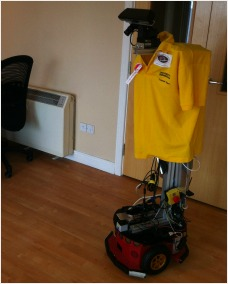
\includegraphics[width=3.in]{dorafinal.jpg}
\caption{Dora robot}
\label{fig:dora}
\end{figure}

\section{Software architecture}
The system is composed of several independent programs/nodes and thus reusable parts of code with different functionality. The different nodes communicate between them by exchanging ROS messages and ROS actions \ref{fig:nodes}. The core element of our framework that binds the rest of the node/processes together is a state machine node. (needs heavy editing this part)

\begin{figure}[!t]
\centering
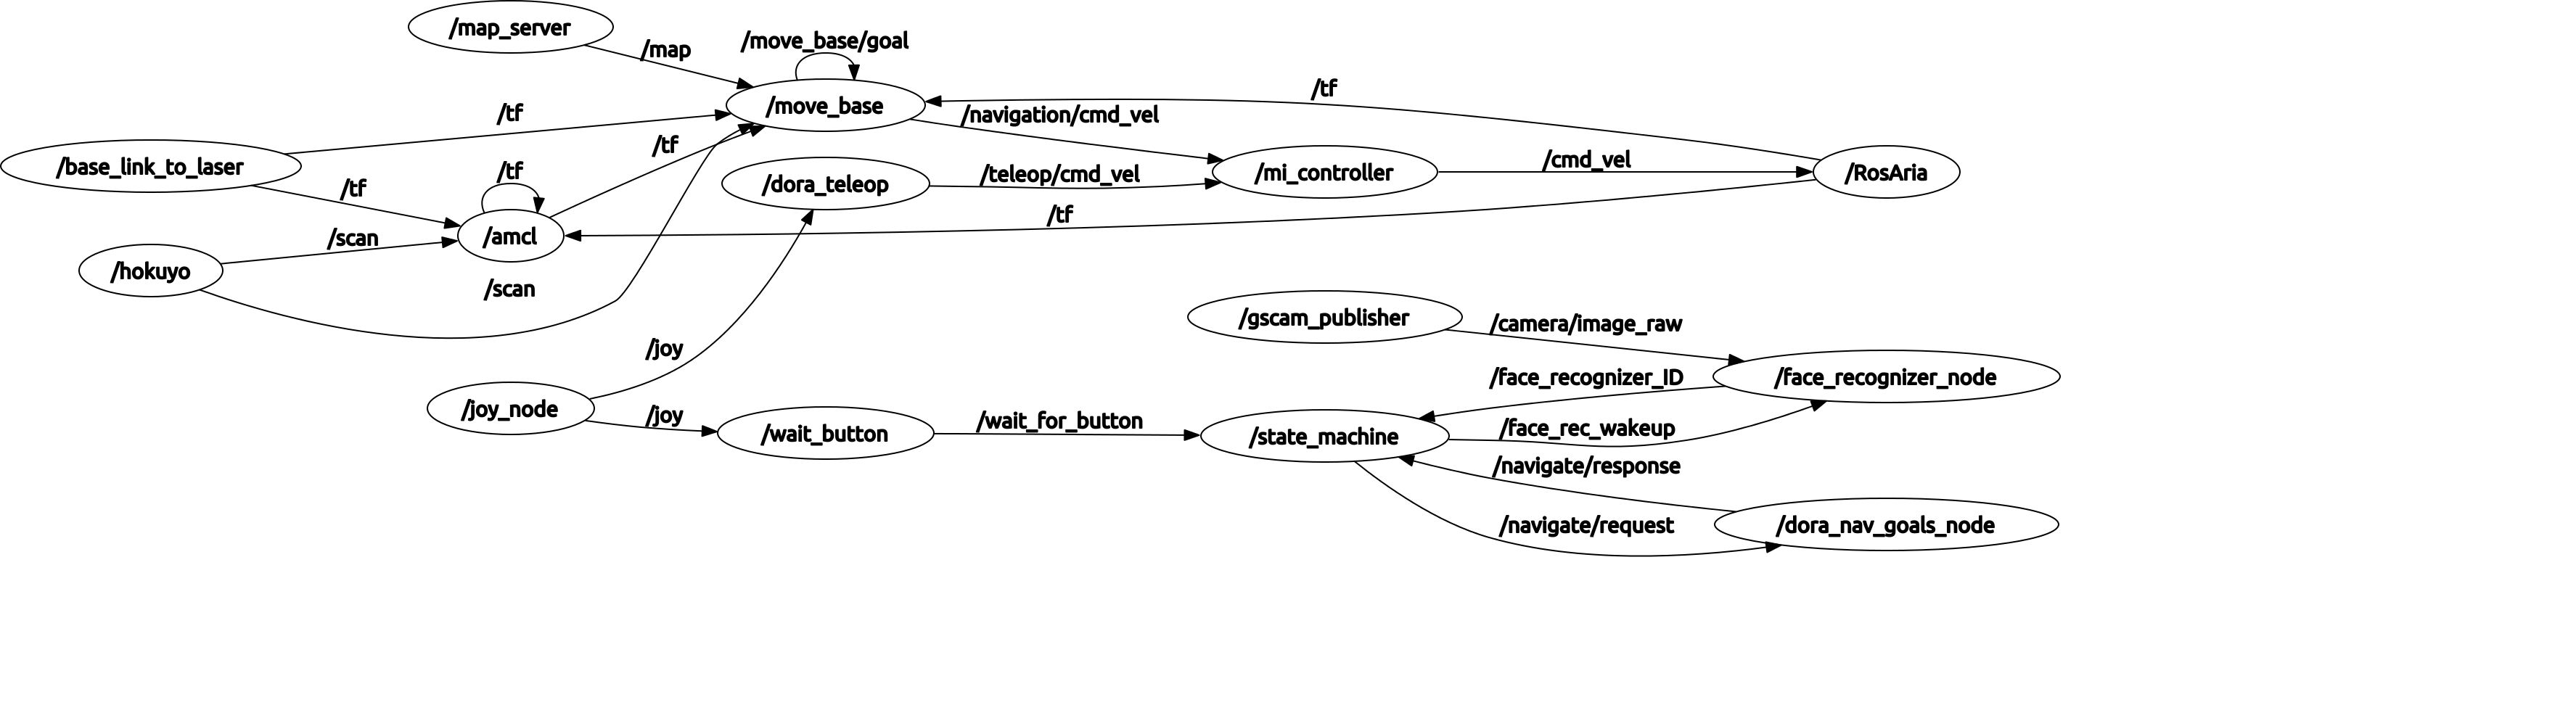
\includegraphics[width=4.in]{nodes.png}
\caption{An overview of the software architecture and how the nodes are connected interact with each other}
\label{fig:nodes}
\end{figure}

\subsection{Middleware-Robot Operating System}
Robot Operating System (ROS) (cite here) will be used as the middleware. ROS open source philosophy is powerful and allows code re-usability by different programmers. It allows us to use robust, state of the art or our own AI algorithms without worrying about how to write code for low level motor commands or sensor drivers. Even more important is the fact that can save valuable time that otherwise would be spend in merging different architectures or worrying of how different pieces of software would communicate with each other. Lastly, ROS was also chosen as it has become almost a standard choice for researchers and thus our lab has extensive hands on experience.

\subsection{State machine}
The core element of our framework that binds the rest of the node/processes together is a state machine node. It is responsible for monitoring the state of the robot and the world. Also it is responsible for deciding what is going to be the next robot action. It was developed with ROS SMACH framework and it works by....

\subsection{Building the map with SLAM}
Since the map is it assumed to be known there is a need to build it before further tests can be done. For initially building a map we made use of the OpenSlam's GMapping algorithm \cite{slam} through the ROS wrapper package called slam gmapping. This approach uses a Rao-Blackwellized particle filter in which each particle carries an individual map of the environment.  The particles are updated by taking into account both odometry and the latests observations from a laser range finder.

\subsection{Localising in a known map with adaptive Monte Carlo localisation}
After the map is known and saved, an Adaptive Monte Carlo Localisation (AMCL)\cite{amcl} algorithm (is part of the ROS navigation stack - see navigation section) is used to localise the robot inside the known environment. It uses laser range finder readings to update a particle filter. Every particle is representing a specific discrete state and stores the uncertainty of robot being in that state/position within the known map. Also every time the robot moves uses the motor information to shift the particles to the corresponding direction. The robot's pose estimate is then been published through a ROS topic for use with other nodes.

\subsection{Navigation}
For navigation and obstacle avoidance, ROS navigation stack is used. It is a proven robust solution for domestic environments (citation here of marathon). More specifically navigation stack reads the odometry, the pose estimate and laser range finder scans from the relevant topics and drives safety the robot inside the environment to some goal. The goal is represented by some given coordinates. For example it drives the robot to the door coordinates, where the robot should perform its face recognition to the person ringing the bell. For achiving this it make use of a global and a local planer. The global planner creates an optimal global path based on robot's pose and a global costmap. Then a local planner, making use of the Dynamic Window Approach algorithm (citation here), is responsible for following that global path and reactively avoiding obstacles.

\subsection{Mixed initiative controller and teleoperation}
These nodes were made as part of another project involving mixed initiative HRI in emergency response robots. Thus, the name is not representative of their exact functionality in this case. The controller it is used to decide which velocity commands to give to the motors whenever some coupling of commands is needed. On one hand are the motor commands coming from robot's AI (e.g. AI navigation) and on the other hand are motor commands coming from a teleoperation node and a human through a joystick. Although the robot is autonomous, the latter is necessary as the user needs to place the robot in the initial state, move it around during testing just by pausing AI commands, or stop the robot in the case of an emergency (e.g. robot repeatedly hitting a wall, so the user has to stop it and drive it away).  This is another example of code which can be reused in many different applications.

\subsection{Dora navigation goals node}

\subsection{Face detection and recognition}
In order to improve the HRI skills of the robot we have implemented in our system face detection and face recognition capabilities (see FIG.\ref{fig:face}). The first one is used to find candidate face patterns inside an image, while the latter tries to find the best match of a new face with a known dataset.

Face detection is performed using the Viola-Jones algorithm \cite{Viola01_RapidObjDet}. The algorithm uses a supervised machine learning approach, where a cascade function is trained with many positive and negative images. Then, it is used to detect faces in other images. The algorithm uses many simple Haar feature classifiers which are applied incrementally in different regions of the image in order to discriminate candidate face regions. One of these feature classifiers won't identify a face just by itself, but the combined and supplementary use of all the simple Haar classifiers succeeds.

Face recognition is performed by applying a Local Binary Pattern Histogram (LBPH) algorithm \cite{Ahonen04_FaceRecLBP}.  The principle is to build local binary patterns (LBP) for each pixel depending on a variable neighbourhood scheme. Then, divide the formed LBP image into m local regions and extract the histogram from each. Finally, classification is performed by comparing the resulting histograms with the ones of the classes in the dataset.

\begin{figure}[!t]
\centering
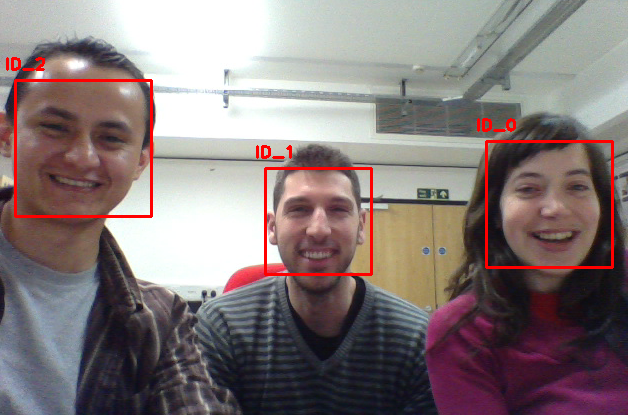
\includegraphics[width=3.in]{BARC_FaceRec.png}
\caption{An example of the face detection and face recognition algorithms. The red bounding boxes surround the successfully detected faces, while each of them is given a corresponding identification code.}
\label{fig:face}
\end{figure}

\subsection{Transformations}

\section{Future work}
%and maybe enlargements?
%from rules: Applicability and relevance to domestic/industrial robotics [@Home / @Work]


% An example of a floating figure using the graphicx package.
% Note that \label must occur AFTER (or within) \caption.
% For figures, \caption should occur after the \includegraphics.
% Note that IEEEtran v1.7 and later has special internal code that
% is designed to preserve the operation of \label within \caption
% even when the captionsoff option is in effect. However, because
% of issues like this, it may be the safest practice to put all your
% \label just after \caption rather than within \caption{}.
%
% Reminder: the "draftcls" or "draftclsnofoot", not "draft", class
% option should be used if it is desired that the figures are to be
% displayed while in draft mode.
%
%\begin{figure}[!t]
%\centering
%\includegraphics[width=2.5in]{myfigure}
% where an .eps filename suffix will be assumed under latex, 
% and a .pdf suffix will be assumed for pdflatex; or what has been declared
% via \DeclareGraphicsExtensions.
%\caption{Simulation Results}
%\label{fig_sim}
%\end{figure}

% Note that IEEE typically puts floats only at the top, even when this
% results in a large percentage of a column being occupied by floats.


% An example of a double column floating figure using two subfigures.
% (The subfig.sty package must be loaded for this to work.)
% The subfigure \label commands are set within each subfloat command, the
% \label for the overall figure must come after \caption.
% \hfil must be used as a separator to get equal spacing.
% The subfigure.sty package works much the same way, except \subfigure is
% used instead of \subfloat.
%
%\begin{figure*}[!t]
%\centerline{\subfloat[Case I]\includegraphics[width=2.5in]{subfigcase1}%
%\label{fig_first_case}}
%\hfil
%\subfloat[Case II]{\includegraphics[width=2.5in]{subfigcase2}%
%\label{fig_second_case}}}
%\caption{Simulation results}
%\label{fig_sim}
%\end{figure*}
%
% Note that often IEEE papers with subfigures do not employ subfigure
% captions (using the optional argument to \subfloat), but instead will
% reference/describe all of them (a), (b), etc., within the main caption.


% An example of a floating table. Note that, for IEEE style tables, the 
% \caption command should come BEFORE the table. Table text will default to
% \footnotesize as IEEE normally uses this smaller font for tables.
% The \label must come after \caption as always.
%
%\begin{table}[!t]
%% increase table row spacing, adjust to taste
%\renewcommand{\arraystretch}{1.3}
% if using array.sty, it might be a good idea to tweak the value of
% \extrarowheight as needed to properly center the text within the cells
%\caption{An Example of a Table}
%\label{table_example}
%\centering
%% Some packages, such as MDW tools, offer better commands for making tables
%% than the plain LaTeX2e tabular which is used here.
%\begin{tabular}{|c||c|}
%\hline
%One & Two\\
%\hline
%Three & Four\\
%\hline
%\end{tabular}
%\end{table}


% Note that IEEE does not put floats in the very first column - or typically
% anywhere on the first page for that matter. Also, in-text middle ("here")
% positioning is not used. Most IEEE journals/conferences use top floats
% exclusively. Note that, LaTeX2e, unlike IEEE journals/conferences, places
% footnotes above bottom floats. This can be corrected via the \fnbelowfloat
% command of the stfloats package.



\section{Conclusion}
All team members have a strong motivation in participating in the robotic competitions. We think that the RoCKIn@Home will provide interesting challenge for us and it will address the problematic of the real robots in our homes. As a result, we are expecting to obtain more knowledge in the ongoing research in many fields in robotic.

If three our members will be accepted to participate in the RoCKIn camp, we assumed this will help us to get into the demanding robotic topics more faster and produce better and more interesting solution of the overall system.




% conference papers do not normally have an appendix


% use section* for acknowledgement
%\section*{Acknowledgment}



% trigger a \newpage just before the given reference
% number - used to balance the columns on the last page
% adjust value as needed - may need to be readjusted if
% the document is modified later
%\IEEEtriggeratref{8}
% The "triggered" command can be changed if desired:
%\IEEEtriggercmd{\enlargethispage{-5in}}

% references section

% can use a bibliography generated by BibTeX as a .bbl file
% BibTeX documentation can be easily obtained at:
% http://www.ctan.org/tex-archive/biblio/bibtex/contrib/doc/
% The IEEEtran BibTeX style support page is at:
% http://www.michaelshell.org/tex/ieeetran/bibtex/


\bibliographystyle{IEEEtran}
\bibliography{./ref}
%
% <OR> manually copy in the resultant .bbl file
% set second argument of \begin to the number of references
% (used to reserve space for the reference number labels box)
%\begin{thebibliography}{1}

%\bibitem{IEEEhowto:kopka}
%H.~Kopka and P.~W. Daly, \emph{A Guide to \LaTeX}, 3rd~ed.\hskip 1em plus
%0.5em minus 0.4em\relax Harlow, England: Addison-Wesley, 1999.

%\end{thebibliography}




% that's all folks
\end{document}


